% TO-DO:  Kolmogorov complexity

\documentclass[17pt]{beamer}
\usepackage[CJKspace]{xeCJK}
%\usepackage{newtxtext,newtxmath}	% use Times Roman font
%\usefonttheme{serif}
\usefonttheme{professionalfonts}
%\setbeamertemplate{theorems}[numbered]
\setbeamertemplate{caption}{\insertcaption} 	% no `Figure' prefix before caption

\mode<presentation> {

%\usetheme{default}
%\usetheme{AnnArbor}
%\usetheme{Antibes}
%\usetheme{Bergen}
%\usetheme{Berkeley}
%\usetheme{Berlin}
%\usetheme{Boadilla}
%\usetheme{CambridgeUS}
%\usetheme{Copenhagen}
%\usetheme{Darmstadt}
%\usetheme{Dresden}
%\usetheme{Frankfurt}
%\usetheme{Goettingen}
%\usetheme{Hannover}
%\usetheme{Ilmenau}
%\usetheme{JuanLesPins}
%\usetheme{Luebeck}
\usetheme{Madrid}
%\usetheme{Malmoe}
%\usetheme{Marburg}
%\usetheme{Montpellier}
%\usetheme{PaloAlto}
%\usetheme{Pittsburgh}
%\usetheme{Rochester}
%\usetheme{Singapore}
%\usetheme{Szeged}
%\usetheme{Warsaw}

%\usecolortheme{albatross}
%\usecolortheme{beaver}
%\usecolortheme{beetle}
%\usecolortheme{crane}
%\usecolortheme{dolphin}
%\usecolortheme{dove}
%\usecolortheme{fly}
%\usecolortheme{lily}
%\usecolortheme{orchid}
%\usecolortheme{rose}
%\usecolortheme{seagull}
%\usecolortheme{seahorse}
%\usecolortheme{whale}
%\usecolortheme{wolverine}

%\setbeamertemplate{footline} % To remove the footer line in all slides uncomment this line
%\setbeamertemplate{footline}[page number] % To replace the footer line in all slides with a simple slide count uncomment this line
\setbeamertemplate{navigation symbols}{} % To remove the navigation symbols from the bottom of all slides uncomment this line
}

\renewcommand\textbullet{\leavevmode%
	\usebeamertemplate{itemize item}\hspace{.5em}}

\usepackage{graphicx} % Allows including images
\usepackage{verbatim} % comments
% \usepackage{tikz-cd}  % commutative diagrams
% \newcommand{\tikzmark}[1]{\tikz[overlay,remember picture] \node (#1) {};}
% \usepackage{booktabs} % Allows the use of \toprule, \midrule and \bottomrule in tables
% \usepackage{amssymb}  % \leftrightharpoons
\usepackage{wasysym} % frownie face
\usepackage[makeroom]{cancel}	% cross out

\newcommand{\vect}[1]{\boldsymbol{#1}}
\newcommand*\sigmoid{\vcenter{\hbox{
\includegraphics{sigmoid.png}}}}

\makeatletter
\renewcommand{\boxed}[1]{\fbox{\m@th$\displaystyle\scalebox{0.9}{#1}$} \,}
\makeatother

%---------------------------- make slide margin narrower --------------------------------
\newcommand\Wider[2][3em]{%
	\makebox[\linewidth][c]{%
		\begin{minipage}{\dimexpr\textwidth+#1\relax}
			\raggedright#2
		\end{minipage}%
}%
}

%----------------------------------------------------------------------------------------
%	TITLE PAGE
%----------------------------------------------------------------------------------------

\title[Logic AI]{{\normalsize 不要再怪我没教你:}\\ Logic-based AI 入门} % The short title appears at the bottom of every slide, the full title is only on the title page

\author{YKY 甄景贤} % Your name
\institute[] % Your institution as it will appear on the bottom of every slide, may be shorthand to save space
{
Independent researcher, Hong Kong \\ % Your institution for the title page
\medskip
\textit{generic.intelligence@gmail.com} % Your email address
}
\date{\today} % Date, can be changed to a custom date

\begin{document}

\frame{\titlepage}

\begin{frame}
\frametitle{Talk summary}
\tableofcontents
\end{frame}

%---------------- this is for when you're using \part's ----------------------------------
%\begin{frame}
%\frametitle{Summary}
%
%{\usebeamerfont*{frametitle} Part I %\usebeamercolor[fg]{frametitle}
% ~ ~ ~ Deep reinforcement learning}
%%\tableofcontents[part=1]
%
%\vspace{1.5cm}
%{\usebeamerfont*{frametitle} Part II %\usebeamercolor[fg]{frametitle}
% ~ ~ ~ Logical structure}
%%\tableofcontents[part=2]
%\end{frame}

%----------------------------------------------------------------------------------------
%	PRESENTATION SLIDES
%----------------------------------------------------------------------------------------

%------------------------------------------------

%\part{title}

% \fontsize{16}{15}\selectfont

\section[Section]{历史}
\frame{\sectionpage}

\begin{frame}
\frametitle{Aristotle (ca. 300BC)}
\textbullet 逻辑 是 研究 (人类) {\color{red} \ 思考方式} 的学问
\fontsize{16}{16}\selectfont
\begin{minipage}[t]{0.5\linewidth}
	\begin{itemize}
		\item 亚里士多德 研究\\
			三段论 (syllogism)
		\item eg: \\
			所有人都会死 \\
			苏格拉底 是人 \\
			$\Rightarrow$ 苏格拉底 会死
	\end{itemize}
\end{minipage}
\hfill
\begin{minipage}[t]{0.45\linewidth}
	\begin{figure}[H]
		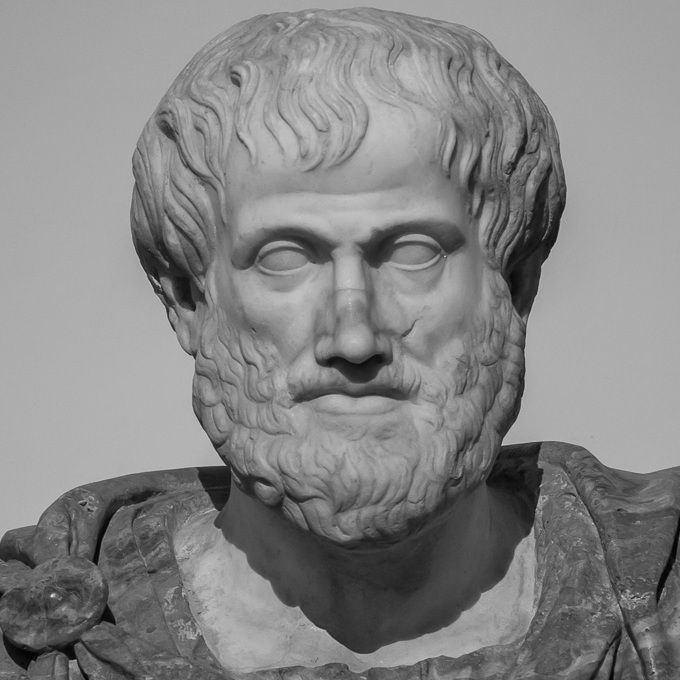
\includegraphics[scale=0.25]{Aristotle.jpg}
	\end{figure}
\end{minipage}
\end{frame}

\begin{frame}
\frametitle{Leibniz (1646-1716)}
\fontsize{15}{15}\selectfont
\begin{minipage}[t]{0.6\linewidth}
	\begin{itemize}
		\item 他预言 在未来 人类的争论 可以 用数学逻辑 透过 {\color{red}\ 计算} 解决 (\textit{calculus ratiocinator})
		\item 逻辑学中的大部分规律,早已在他的著作中出现
		\item 可惜著作失传,直到近代才翻译,对逻辑学发展的影响不大
	\end{itemize}
\end{minipage}
\hfill
\begin{minipage}[t]{0.35\linewidth}
	\begin{figure}[H]
		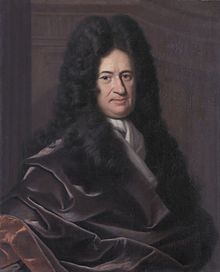
\includegraphics[scale=1.25]{Leibniz.jpg}
	\end{figure}
\end{minipage}
\end{frame}

\begin{frame}
\frametitle{George Boole (1815-1864)}
\fontsize{16}{16}\selectfont
\begin{minipage}[t]{0.6\linewidth}
	\begin{itemize}
		\item 企图用 {\color{red} \ 代数} (algebra) 模拟 逻辑
		\item eg: $x =$ 人, $y =$ 动物 \\
		$\quad xy =$ 人是动物
		\item 他发明的逻辑 和我们今天讲的 Boolean 代数有些不同
	\end{itemize}
\end{minipage}
\hfill
\begin{minipage}[t]{0.35\linewidth}
	\begin{figure}[H]
		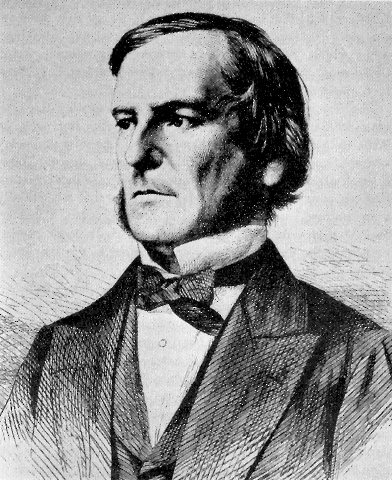
\includegraphics[scale=1.0]{Boole.jpg}
	\end{figure}
\end{minipage}
\end{frame}

\begin{frame}
\frametitle{Gottlob Frege (1848-1925)}
\fontsize{15}{15}\selectfont
\begin{minipage}[t]{0.55\linewidth}
	\begin{itemize}
		\item 发明 {\color{red}\ predicate logic} (谓词逻辑),第一种可以表述大部份思想/语言的逻辑
		\item Russell 写信告诉他,他的逻辑中存在 \textbf{悖论} (paradox)
		\item 他说:「一个作者最惨就是,正当付梓印刷时,才发现书的基础有问题」!
	\end{itemize}
\end{minipage}
\hfill
\begin{minipage}[t]{0.4\linewidth}
	\begin{figure}[H]
		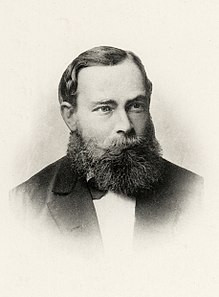
\includegraphics[scale=0.55]{Frege.jpg}
	\end{figure}
\end{minipage}
\end{frame}

\begin{frame}
\frametitle{Principia Mathematica (1910's)}
\fontsize{16}{16}\selectfont
\begin{minipage}[t]{0.35\linewidth}
	\begin{itemize}
		\item Russell \& Whitehead 巨著
		\item 奠定了 \\
		{\color{red}谓词逻辑} \\
		在 数学 中的地位
	\end{itemize}
\end{minipage}
\hfill
\begin{minipage}[t]{0.61\linewidth}
	\begin{figure}[H]
		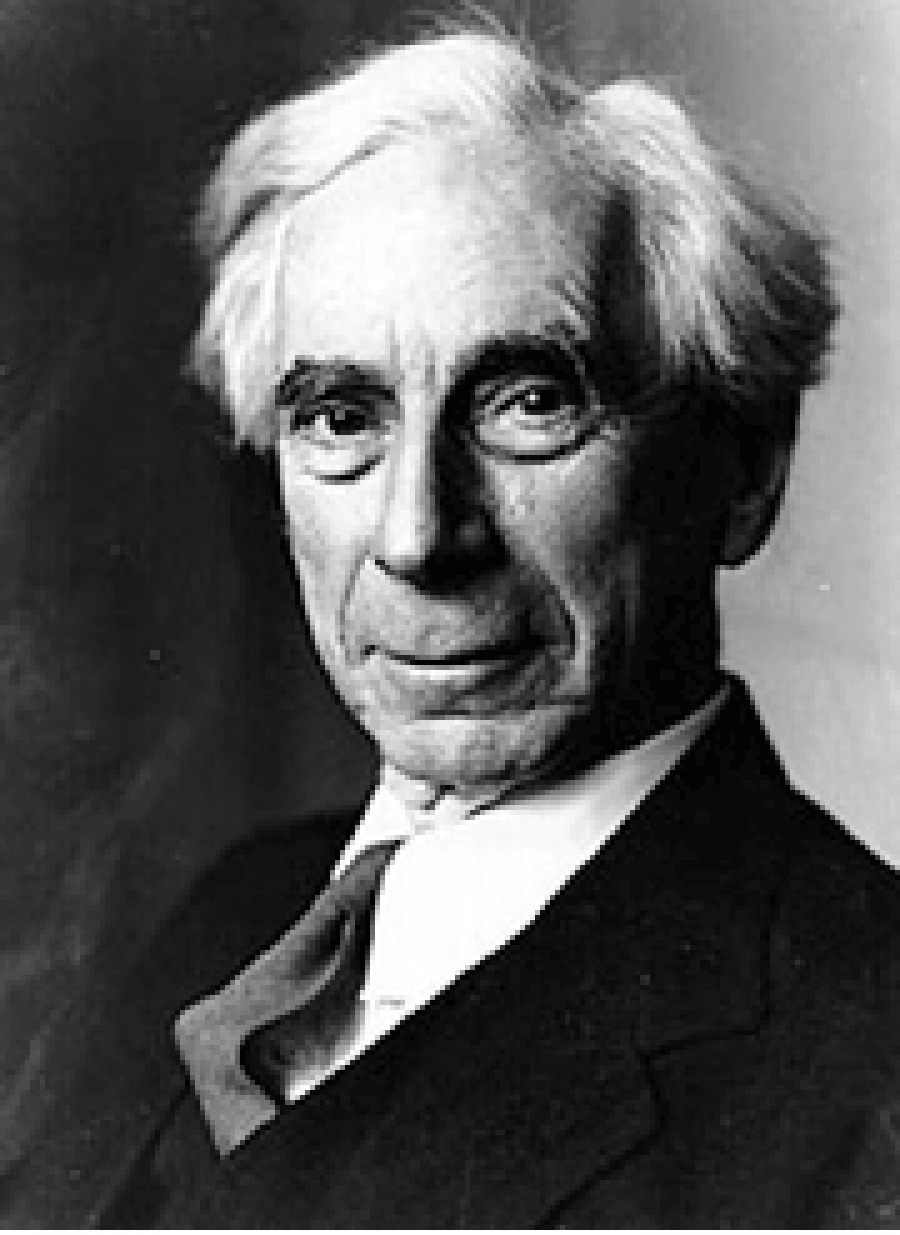
\includegraphics[scale=0.1]{Russell.jpg}
		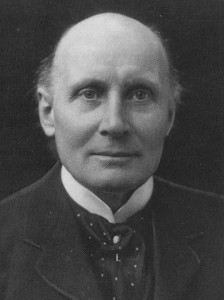
\includegraphics[scale=0.4]{Whitehead.jpg}
	\end{figure}
	\vspace{1em}
\end{minipage}
\textbullet John McCarthy 在 1950's 将 数理逻辑 引入 {\color{red} \ AI}
\end{frame}

\begin{frame}
\frametitle{Emil Post (1897-1954)}
\fontsize{16}{16}\selectfont
\begin{minipage}[t]{0.62\linewidth}
	\begin{itemize}
		\item 犹太裔 天才儿童
		\item 12 岁时 车祸 失去左臂
		\item 开创 \textbf{递归论}、\textbf{可计算性} 理论
		\item 得到比 G\"{o}del 先的结果,但没有发表
		\item Manic-depressive 精神病
		\item 接受 电击疗法 时 心脏病发致死,死时57岁
	\end{itemize}
\end{minipage}
\hfill
\begin{minipage}[t]{0.35\linewidth}
	\begin{figure}[H]
		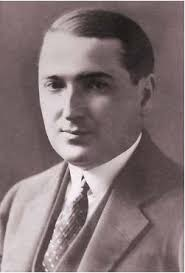
\includegraphics[scale=0.5]{Post.jpg}
	\end{figure}
\end{minipage}
\end{frame}

\begin{frame}
\frametitle{Haskell Curry (1900-1982)}
\fontsize{16}{16}\selectfont
\begin{minipage}[t]{0.62\linewidth}
	\begin{itemize}
		\item 他的姓和名 都变成了 \\编程语言!
		\item 发展 {\color{red} \ combinatory logic},一种不需 \textbf{变量} 的逻辑
		\item Currying 的意思是 $f(x,y)$ 变成 $\hat{f}(x)(y)$
		\item Curry-Howard correspondence: \\
			{\color{red}逻辑推导} 与 {\color{red}\ 计算} \\
			之间的等价关系
	\end{itemize}
\end{minipage}
\hfill
\begin{minipage}[t]{0.35\linewidth}
	\begin{figure}[H]
		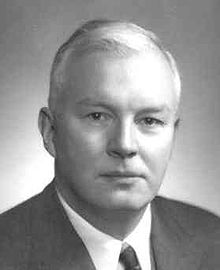
\includegraphics[scale=0.5]{Curry.jpg}
	\end{figure}
\end{minipage}
\end{frame}

\begin{frame}
\frametitle{Alfred Tarski (1901-1983)}
\fontsize{16}{16}\selectfont
\begin{minipage}[t]{0.62\linewidth}
	\begin{itemize}
		\item 开创 {\color{red} \ 模型论} \\ (model theory)
		\item 开创 {\color{red} \ cylindric algebra}, \\
		揭示 谓词逻辑 的 代数/几何 结构
		\item 研究 theory of truth \\
		(这部分我不太清楚)
	\end{itemize}
\end{minipage}
\hfill
\begin{minipage}[t]{0.35\linewidth}
	\begin{figure}[H]
		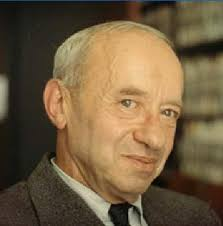
\includegraphics[scale=0.5]{Tarski.jpg}
	\end{figure}
\end{minipage}
\end{frame}

\begin{frame}
\frametitle{Alonzo Church (1903-1995)}
\fontsize{16}{16}\selectfont
\begin{minipage}[t]{0.55\linewidth}
	\begin{itemize}
		\item 发明 {\color{red} \ $\lambda-$calculus}
		\item 目的是研究 {\color{red} \ 代入} (substitution) 的机制
		\item 是任何 {\color{red} \ 可计算函数} 的 \textbf{universal form}\\
		(此即 Church-Turing hypothesis)
	\end{itemize}
\end{minipage}
\hfill
\begin{minipage}[t]{0.4\linewidth}
	\begin{figure}[H]
		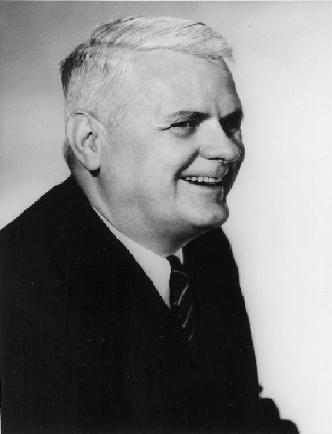
\includegraphics[scale=0.4]{Church.jpg}
	\end{figure}
\end{minipage}
\end{frame}

\begin{frame}
\frametitle{Kurt G\"{o}del (1906-1978)}
\fontsize{14}{14}\selectfont
\begin{minipage}[t]{0.62\linewidth}
	\begin{itemize}
		\item 受 纳粹 逼害,逃到美国
		\item 晚年有 被害妄想症,怕被人下毒,只吃妻子煮的食物
		\item 妻子是护士,有一次她生病入院6个月,结果 G\"{o}del 在家{\color{red}饿死}了!
		\item \textbf{不完备性} (incompleteness) 似乎不妨碍 AGI 的发展 \\
			\vspace{0.5em} \textrm{``not a show-stopper''}
	\end{itemize}
\end{minipage}
\hfill
\begin{minipage}[t]{0.35\linewidth}
	\begin{figure}[H]
		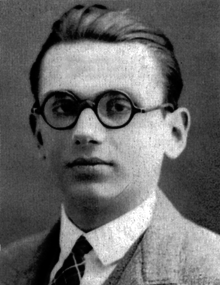
\includegraphics[scale=0.5]{Godel.png}
	\end{figure}
\end{minipage}
\end{frame}

\begin{frame}
\frametitle{Richard Montague (1930-1971)}
\fontsize{14}{14}\selectfont
\begin{minipage}[t]{0.62\linewidth}
	\begin{itemize}
		\item Tarski 的学生
		\item 将英语语法的一个 fragment 转译成 谓词逻辑
		\item 由此证明了 {\color{red}\ 自然语言} 可以 翻译成 {\color{red}\ 逻辑}(形式语义学)
		\item 同性恋者,喜欢 性派对
		\item 某次他带了 3-4 人回家,第二天被发现勒死在浴室,死时40岁
		\item 疑犯将他的汽车撞毁并焚烧
		\item 这案件至今未侦破
	\end{itemize}
\end{minipage}
\hfill
\begin{minipage}[t]{0.35\linewidth}
	\begin{figure}[H]
		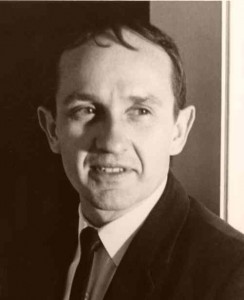
\includegraphics[scale=0.5]{Montague.jpg}
	\end{figure}
\end{minipage}
\end{frame}

\section[Section]{绪论}
\frame{\sectionpage}

\begin{frame}
\frametitle{为什么要学 logic-based AI?}
\begin{itemize}
	\item \textbf{神经网络/深度学习} 是现时 (2019) 最强的学习算法
	\item 某种意义上说,逻辑 AI 已经 \textbf{过时}
	\item 很多人(包括外国)不熟悉 逻辑 AI,所以看不懂我的 理论,还有 OpenCog、OpenNARS 这些「第一代」AGI
	\item 逻辑 是 强人工智能 的基础
\end{itemize}
\end{frame}

\begin{frame}
\frametitle{什么是「命题」?}
\begin{itemize}
	\item 命题 是 任何可以 {\color{red}\ 赋予 真值} 的表达式
	\item 「山楂饼」不是命题
	\item 「我爱吃山楂饼」是命题
	\item 命题 由 {\color{red}\ 概念} (concepts) 组合而成
\end{itemize}
以上似乎是 逻辑 最基本的 预设
\end{frame}

\begin{frame}
\frametitle{反对 逻辑, 论点 \#1}
有没有 不能用 逻辑 表达的思想 (thoughts)?
\begin{itemize}
\item 如果有,你必须把它用文字表述出来
\item 基本上,任何语言表述 可以 转化成 逻辑形式
\item 所以,一定讲不出来
\end{itemize}
事实上,一些足够强的逻辑,包括一阶谓词逻辑,已经可以表达任何 可计算函数
\end{frame}

\begin{frame}
\frametitle{神经网络 vs 逻辑}
\begin{itemize}
	\item 
\end{itemize}
\end{frame}

\begin{frame}
\frametitle{反对 逻辑, 论点 \#2}

\begin{itemize}
	\item
\end{itemize}
\end{frame}

\section[Section]{更多 逻辑 理论}
\frame{\sectionpage}

\begin{frame}
\frametitle{命题逻辑 vs 谓词逻辑}
\begin{itemize}
	\item blah
\end{itemize}
\end{frame}

\begin{frame}
\frametitle{一阶逻辑 vs 二阶/高阶逻辑}
\begin{itemize}
	\item blah
\end{itemize}
\end{frame}


\begin{frame}
\frametitle{范畴 逻辑 (categorical logic)}
\begin{itemize}
	\item blah
\end{itemize}
\end{frame}

\begin{frame}
\frametitle{}
\begin{itemize}
	\item blah
\end{itemize}
\end{frame}

\section[Section]{逻辑AI系统 的 架构}
\frame{\sectionpage}

\begin{frame}
\frametitle{}
\begin{itemize}
	\item blah
\end{itemize}
\end{frame}


\begin{frame}
\frametitle{Rules 和 facts 的區別}
\begin{itemize}
	\item blah
\end{itemize}
\end{frame}



\begin{frame}
\frametitle{}
\begin{itemize}
	\item blah
\end{itemize}
\end{frame}

\section[Section]{推导 算法}
\frame{\sectionpage}

\begin{frame}
\frametitle{消解 (resolution) 算法}
\begin{itemize}
	\item 1965 年 J A Robinson 发明
	\item 命题 {\color{red}\ 推导} (deduction) 的基本算法
	\item 在一堆 conjunctions 之中,将两个 \textbf{互补} 的项消去,例如 $A$ 和 $\neg A$
	\item $\cancel{\color{red}\neg A} \vee B, \cancel{\color{red}A} \vee B \Rightarrow B$
	\item 可以将欲推导的 结论 反转,加入前提中,再用消解法 导出矛盾(反证法)
\end{itemize}
\end{frame}

\begin{frame}
\frametitle{消解 (resolution) 算法(例子)}
\begin{itemize}
	\item 移民外国,寄人篱下,活得没有尊严 $\rightarrow$ 惨
	\item 留在本国,制度压抑,不能舒展抱负 $\rightarrow$ 惨
	\item $A \rightarrow B \equiv \neg A \vee B$ 所以有:
	\item $\cancel{\color{red}\neg\mbox{移民}} \vee \mbox{惨}, \cancel{\color{red}\mbox{移民}} \vee \mbox{惨} \Rightarrow \mbox{惨}$
	\item 移民也惨,不移民也惨 $\Rightarrow$ 惨!
\end{itemize}
\end{frame}

\begin{frame}
\frametitle{同一化 (unification) 算法}
\begin{itemize}
	\item 
\end{itemize}
\end{frame}

\begin{frame}
\frametitle{加速: ``rete'' 算法}
\begin{itemize}
	\item 
\end{itemize}
\end{frame}


\section[Section]{概率/模糊 逻辑}
\frame{\sectionpage}

\begin{frame}
\frametitle{贝叶斯 (Bayesian) 网络}
\begin{itemize}
	\item blah
\end{itemize}
\end{frame}

\begin{frame}
\frametitle{}
\begin{itemize}
	\item blah
\end{itemize}
\end{frame}

\begin{frame}
\frametitle{}
\begin{itemize}
	\item blah
\end{itemize}
\end{frame}

\section[Section]{学习 算法}
\frame{\sectionpage}

\begin{frame}
\frametitle{}
\begin{itemize}
	\item blah
\end{itemize}
\end{frame}

\begin{frame}
\frametitle{}
\begin{itemize}
	\item blah
\end{itemize}
\end{frame}

\section*{结论}

\begin{frame}
\frametitle{?}
\Wider[1em]{
\begin{itemize}
	\item
\end{itemize}
}
	\begin{center}
		多谢收看 \smiley{}
	\end{center}
\end{frame}

\begin{comment}

\begin{frame}
\frametitle{References}
\footnotesize{
\begin{thebibliography}{99} % Beamer does not support BibTeX so references must be inserted manually as below
\bibitem[]{} Bart Jacobs (1999)
\newblock Categorical logic and type theory
% \newblock \emph{North Holland, Studies in logic} v141.

\bibitem[]{} Robert Goldblatt (2006)
\newblock Topoi -- the categorical analysis of logic

\end{thebibliography}
}
\end{frame}

\begin{frame}
We're looking for developers to implement a prototype.

\vspace*{1cm}
\Large{\centerline{Thank you}}

%\vspace*{1cm}
%\Large{\centerline{The End}}
\end{frame}

\end{comment}

\end{document} 